\documentclass[11pt,a4paper]{article}
\usepackage[utf8]{inputenc}
\usepackage[vietnamese]{babel}
\usepackage{amsmath,amssymb}
\usepackage[version=4]{mhchem}
\usepackage{geometry}
\geometry{top=1.5cm,bottom=1.2cm,left=1.4cm,right=1.4cm,headheight=28pt,headsep=12pt,footskip=18pt}
\usepackage{graphicx}
\usepackage{xcolor}
\usepackage{tabularx}
\usepackage{array}
\usepackage{tikz}
\usepackage{fancyhdr}
\usepackage{enumitem}
\usepackage{multido}
\usepackage{tcolorbox}
\usepackage{colortbl}

\definecolor{hfRed}{HTML}{D32F2F}
\definecolor{hfGreen}{HTML}{8BC390}
\definecolor{mainGreen}{HTML}{2E7D32}
\definecolor{solBlue}{HTML}{1565C0}
\definecolor{tableGreen}{HTML}{E8F5E9}

\usepackage{ex_test}

\pagestyle{fancy}
\fancyhf{}
\renewcommand{\headrulewidth}{0.75pt}
\renewcommand{\headrule}{\hbox to\headwidth{\color{hfGreen}\leaders\hrule height \headrulewidth\hfill}}
\renewcommand{\footrulewidth}{0.75pt}
\renewcommand{\footrule}{\hbox to\headwidth{\color{hfGreen}\leaders\hrule height \footrulewidth\hfill}}

\fancyhead[L]{\small\itshape\color{hfRed}Tài liệu lưu hành nội bộ}
\fancyhead[R]{\small\color{hfRed}Thầy \textbf{TRẦN VĂN THẠNH} - 0777.470.803}

\fancyfoot[L]{\footnotesize\itshape\color{hfRed}CS1: 6/15 Nguyễn Hoàng, P. Kim Long, TP Huế \quad|\quad CS2: 24 Đặng Thái Thân, TP Huế}
\fancyfoot[R]{\small\textbf{\color{hfRed}Trang \thepage}}

\setlength{\parindent}{0pt}
\setlength{\parskip}{2pt}

\begin{document}

\begin{minipage}[t]{0.48\textwidth}
\textbf{SỞ GD\&ĐT THÀNH PHỐ HUẾ}\\
\textbf{TRƯỜNG THPT NGUYỄN CHÍ THANH}\\
\textit{ĐỀ CHÍNH THỨC}\\
\textit{(Đề có 04 trang)}
\end{minipage}
\hfill
\begin{minipage}[t]{0.48\textwidth}
\raggedleft
\textbf{\color{hfRed}ĐỀ KIỂM TRA GIỮA HỌC KỲ I – NĂM HỌC 2026 – 2027}\\
\textbf{MÔN HOÁ HỌC - LỚP 10}\\
\textit{Thời gian làm bài: 45 phút (không kể thời gian phát đề)}\\
\textbf{Mã đề: 1104}
\end{minipage}

\vspace{4pt}
\noindent
\textit{Họ tên:} \dotfill \textit{Lớp:} \dotfill \textit{Số báo danh:} \dotfill

\vspace{2pt}
\noindent
\textit{\footnotesize Cho biết nguyên tử khối (amu): $\ce{H = 1; C = 12; N = 14; O = 16; Na = 23; Mg = 24; Al = 27; P = 31; S = 32; Cl = 35{,}5; K = 39; Ca = 40; Fe = 56; Cu = 64; Zn = 65; Br = 80}$.\\
Cho biết số hiệu nguyên tử: $\ce{H = 1; Li = 3; C = 6; N = 7; O = 8; F = 9; Ne = 10; Na = 11; Mg = 12; Al = 13; Si = 14; P = 15; S = 16; Cl = 17; Ar = 18; K = 19; Ca = 20; Fe = 26; Cu = 29}$.}

\vspace{2pt}
\hrule color{hfGreen} height 0.5pt

\vspace{4pt}
\begin{center}
\textbf{\color{hfRed}\large (BẢN GIÁO VIÊN -- CÓ LỜI GIẢI CHI TIẾT)}
\end{center}

\vspace{2pt}
\begin{center}
{\color{hfRed}\textbf{\large BẢNG ĐÁP ÁN RÚT GỌN (DÀNH CHO GIÁO VIÊN)}}
\end{center}

\vspace{2pt}
\noindent
\textbf{\color{mainGreen}1. Phần I: Trắc nghiệm nhiều lựa chọn (4,0 điểm - mỗi câu đúng 0,25 điểm)}
\begin{center}
\renewcommand{\arraystretch}{1.2}
\small
\begin{tabular}{|c|c|c|c|c|c|c|c|c|c|c|c|c|c|c|c|c|}
\hline
\rowcolor{tableGreen}
\textbf{Câu} & \textbf{1} & \textbf{2} & \textbf{3} & \textbf{4} & \textbf{5} & \textbf{6} & \textbf{7} & \textbf{8} & \textbf{9} & \textbf{10} & \textbf{11} & \textbf{12} & \textbf{13} & \textbf{14} & \textbf{15} & \textbf{16} \\
\hline
\textbf{Đ/A} & \textbf{\color{hfRed}D} & \textbf{\color{hfRed}C} & \textbf{\color{hfRed}A} & \textbf{\color{hfRed}B} & \textbf{\color{hfRed}A} & \textbf{\color{hfRed}B} & \textbf{\color{hfRed}C} & \textbf{\color{hfRed}D} & \textbf{\color{hfRed}B} & \textbf{\color{hfRed}C} & \textbf{\color{hfRed}A} & \textbf{\color{hfRed}D} & \textbf{\color{hfRed}A} & \textbf{\color{hfRed}C} & \textbf{\color{hfRed}A} & \textbf{\color{hfRed}C} \\
\hline
\end{tabular}
\end{center}

\vspace{2pt}
\noindent
\textbf{\color{mainGreen}2. Phần II: Trắc nghiệm Đúng / Sai (2,0 điểm)}
\begin{center}
\renewcommand{\arraystretch}{1.2}
\begin{tabular}{|c|c|c|c|c|}
\hline
\rowcolor{tableGreen}
\textbf{Câu} & \textbf{Lệnh a)} & \textbf{Lệnh b)} & \textbf{Lệnh c)} & \textbf{Lệnh d)} \\
\hline
\textbf{Câu 1} & \textbf{\color{hfRed}ĐÚNG} & \textbf{\color{hfRed}ĐÚNG} & \textbf{\color{solBlue}SAI} & \textbf{\color{solBlue}SAI} \\
\hline
\textbf{Câu 2} & \textbf{\color{hfRed}ĐÚNG} & \textbf{\color{hfRed}ĐÚNG} & \textbf{\color{hfRed}ĐÚNG} & \textbf{\color{hfRed}ĐÚNG} \\
\hline
\end{tabular}
\end{center}

\vspace{2pt}
\noindent
\textbf{\color{mainGreen}3. Phần III: Trắc nghiệm Trả lời ngắn (1,0 điểm - mỗi câu đúng 0,25 điểm)}
\begin{center}
\renewcommand{\arraystretch}{1.2}
\begin{tabular}{|c|c|c|c|c|}
\hline
\rowcolor{tableGreen}
\textbf{Câu hỏi} & \textbf{Câu 1} & \textbf{Câu 2} & \textbf{Câu 3} & \textbf{Câu 4} \\
\hline
\textbf{Đáp án} & \textbf{\color{hfRed}14} & \textbf{\color{hfRed}3} & \textbf{\color{hfRed}10} & \textbf{\color{hfRed}108} \\
\hline
\end{tabular}
\end{center}

\vspace{4pt}
\hrule color{hfGreen} height 0.5pt

\vspace{4pt}
\noindent
\textbf{\large\color{mainGreen}PHẦN I. Câu trắc nghiệm nhiều phương án lựa chọn: (16 câu – 4 điểm)}

\textit{Thí sinh trả lời từ câu 1 đến câu 16. Mỗi câu thí sinh chỉ chọn một phương án.}
\vspace{4pt}

\begin{ex}%[1104-C1]
Các đồng vị của cùng một nguyên tố hóa học là những nguyên tử có
\choice
{cùng số neutron nhưng khác nhau về số proton.}
{cùng số khối $A$ nhưng khác nhau về số proton.}
{cùng tổng số hạt proton và neutron nhưng khác nhau về số electron.}
{\True cùng số proton nhưng khác nhau về số neutron.}
\begin{loigiai}
Đồng vị của cùng một nguyên tố hóa học là những nguyên tử có cùng số proton nhưng khác nhau về số neutron, do đó có số khối $A$ khác nhau.\\
$\rightarrow$ \textbf{Chọn đáp án D.}
\end{loigiai}
\end{ex}

\begin{ex}%[1104-C2]
Cấu hình electron nguyên tử của potassium ($Z = 19$) là $1s^2 2s^2 2p^6 3s^2 3p^6 4s^1$. Vị trí của potassium trong bảng tuần hoàn là
\choice
{ô số 19, chu kì 4, nhóm IB.}
{ô số 19, chu kì 3, nhóm IA.}
{\True ô số 19, chu kì 4, nhóm IA.}
{ô số 19, chu kì 1, nhóm IVA.}
\begin{loigiai}
Potassium ($Z = 19$): có 19 electron, 4 lớp electron, electron hóa trị là $4s^1$ (nguyên tố s).\\
Vị trí trong bảng tuần hoàn: ô số 19, chu kì 4, nhóm IA.\\
$\rightarrow$ \textbf{Chọn đáp án C.}
\end{loigiai}
\end{ex}

\begin{ex}%[1104-C3]
Nguyên tử của nguyên tố phosphorus có $Z = 15$ và $A = 31$. Số hạt neutron trong nguyên tử phosphorus là
\choice
{\True 16.}
{31.}
{46.}
{15.}
\begin{loigiai}
Số hạt neutron trong nguyên tử phosphorus: $N = A - Z = 31 - 15 = 16$.\\
$\rightarrow$ \textbf{Chọn đáp án A.}
\end{loigiai}
\end{ex}

\begin{ex}%[1104-C4]
Cho các nguyên tử sau: $^{12}_{6}\text{X}$, $^{14}_{7}\text{Y}$, $^{13}_{6}\text{Z}$, $^{16}_{8}\text{T}$. Hai nguyên tử nào là đồng vị của cùng một nguyên tố hóa học?
\choice
{$\text{X}$ và $\text{Y}$.}
{\True $\text{X}$ và $\text{Z}$.}
{$\text{Z}$ và $\text{T}$.}
{$\text{Y}$ và $\text{T}$.}
\begin{loigiai}
Hai nguyên tử $^{12}_{6}\text{X}$ và $^{13}_{6}\text{Z}$ đều có cùng số proton $Z = 6$ (nguyên tố carbon), do đó $\text{X}$ và $\text{Z}$ là hai đồng vị của cùng một nguyên tố hóa học.\\
$\rightarrow$ \textbf{Chọn đáp án B.}
\end{loigiai}
\end{ex}

\begin{ex}%[1104-C5]
Số orbital trong các phân lớp s, p, d lần lượt bằng
\choice
{\True 1, 3, 5.}
{1, 2, 3.}
{1, 2, 4.}
{3, 5, 7.}
\begin{loigiai}
Số orbital trong các phân lớp: phân lớp s có 1 orbital, phân lớp p có 3 orbital, phân lớp d có 5 orbital.\\
$\rightarrow$ \textbf{Chọn đáp án A.}
\end{loigiai}
\end{ex}

\begin{ex}%[1104-C6]
Số electron tối đa có thể chứa trong lớp thứ $n$ (với $n \le 4$) được tính theo công thức là
\choice
{$2n + 1$.}
{\True $2n^2$.}
{$2n$.}
{$n^2$.}
\begin{loigiai}
Số electron tối đa trong lớp thứ $n$ (với $n \le 4$) là $2n^2$.\\
$\rightarrow$ \textbf{Chọn đáp án B.}
\end{loigiai}
\end{ex}

\begin{ex}%[1104-C7]
Kí hiệu chung của nguyên tử là $^{A}_{Z}\text{X}$, trong đó $A$ và $Z$ lần lượt biểu diễn cho
\choice
{số hiệu nguyên tử và số khối.}
{số khối và số neutron.}
{\True số khối và số hiệu nguyên tử.}
{số neutron và số hiệu nguyên tử.}
\begin{loigiai}
Trong kí hiệu nguyên tử $^{A}_{Z}\text{X}$, $A$ là số khối (phía trên bên trái), $Z$ là số hiệu nguyên tử (phía dưới bên trái).\\
$\rightarrow$ \textbf{Chọn đáp án C.}
\end{loigiai}
\end{ex}

\begin{ex}%[1104-C8]
Bảng tuần hoàn các nguyên tố hoá học được sắp xếp không tuân theo nguyên tắc nào sau đây?
\choice
{Các nguyên tố mà nguyên tử có cùng số lớp electron được xếp vào một hàng.}
{Các nguyên tố mà nguyên tử có cùng số electron hoá trị được xếp vào một cột.}
{Các nguyên tố được sắp xếp theo chiều tăng dần của điện tích hạt nhân nguyên tử.}
{\True Các nguyên tố được sắp xếp theo chiều tăng dần khối lượng nguyên tử.}
\begin{loigiai}
Bảng tuần hoàn hiện đại được sắp xếp theo chiều tăng dần của điện tích hạt nhân ($Z$), không phải theo chiều tăng dần khối lượng nguyên tử.\\
$\rightarrow$ \textbf{Chọn đáp án D.}
\end{loigiai}
\end{ex}

\begin{ex}%[1104-C9]
Orbital nguyên tử (AO) là
\choice
{quỹ đạo chuyển động có hình tròn xác định của electron xung quanh hạt nhân.}
{\True khu vực không gian xung quanh hạt nhân mà tại đó xác suất tìm thấy electron là lớn nhất.}
{đám mây hình bầu dục chứa tất cả các electron của nguyên tử.}
{đường tròn trên đó các electron chuyển động với tốc độ không đổi.}
\begin{loigiai}
Orbital nguyên tử (AO) là khu vực không gian xung quanh hạt nhân mà tại đó xác suất tìm thấy electron là lớn nhất (khoảng $90\%$).\\
$\rightarrow$ \textbf{Chọn đáp án B.}
\end{loigiai}
\end{ex}

\begin{ex}%[1104-C10]
Nguyên tố hóa học là tập hợp các nguyên tử có cùng
\choice
{số khối $A$.}
{tổng số proton và neutron.}
{\True số proton.}
{số neutron.}
\begin{loigiai}
Nguyên tố hóa học là tập hợp các nguyên tử có cùng số proton (cùng điện tích hạt nhân).\\
$\rightarrow$ \textbf{Chọn đáp án C.}
\end{loigiai}
\end{ex}

\begin{ex}%[1104-C11]
Đồng có hai đồng vị bền trong tự nhiên là $^{63}_{29}\ce{Cu}$ và $^{65}_{29}\ce{Cu}$. Nguyên tử khối trung bình của đồng là 63,55 (điện tích $z$ của các ion đồng vị bền đều bằng $+1$). Hình vẽ phổ khối nào dưới đây là đúng?
\begin{center}
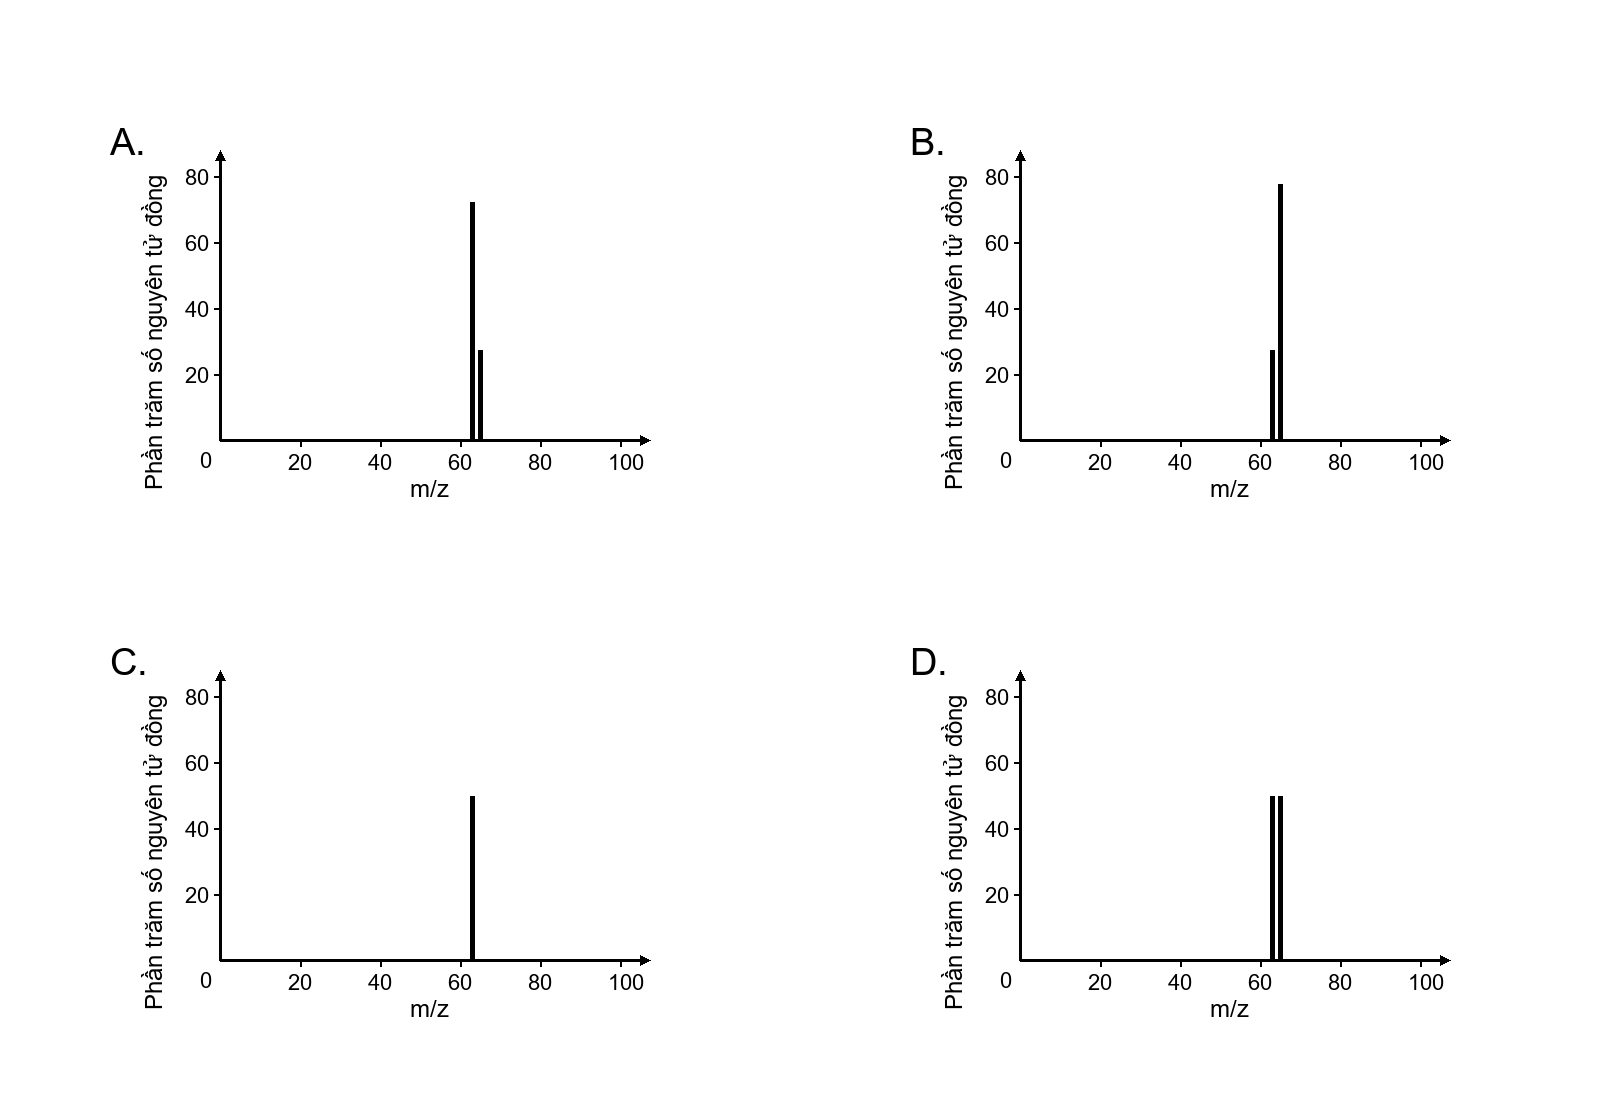
\includegraphics[width=13.5cm]{images_hoa10/pho_khoi_cu_ma1104.png}
\end{center}
\choice
{\True Hình A.}
{Hình B.}
{Hình C.}
{Hình D.}
\begin{loigiai}
Áp dụng công thức nguyên tử khối trung bình:
$$\bar{A} = \dfrac{63x + 65(100 - x)}{100} = 63{,}55 \Rightarrow x = 72{,}5\%$$
Vậy đồng vị $^{63}\ce{Cu}$ chiếm $72{,}5\%$ và $^{65}\ce{Cu}$ chiếm $27{,}5\%$.\\
Do $z = +1$ nên tỉ số $m/z$ lần lượt là $63$ và $65$. Trên phổ khối lượng, pic tại $m/z = 63$ cao $72{,}5\%$ và pic tại $m/z = 65$ cao $27{,}5\%$ tương ứng với Hình A.\\
$\rightarrow$ \textbf{Chọn đáp án A.}
\end{loigiai}
\end{ex}

\begin{ex}%[1104-C12]
Trong nguyên tử, loại hạt nào có khối lượng không đáng kể so với các hạt còn lại?
\choice
{Neutron.}
{Proton.}
{Neutron và electron.}
{\True Electron.}
\begin{loigiai}
Khối lượng của electron ($m_\text{e} \approx 0{,}00055\,\text{amu}$) rất nhỏ so với proton và neutron ($m_\text{p} \approx m_\text{n} \approx 1\,\text{amu}$), nên khối lượng electron được coi là không đáng kể.\\
$\rightarrow$ \textbf{Chọn đáp án D.}
\end{loigiai}
\end{ex}

\begin{ex}%[1104-C13]
Bảng tuần hoàn hiện nay gồm có bao nhiêu chu kì?
\choice
{\True 7.}
{18.}
{8.}
{6.}
\begin{loigiai}
Bảng tuần hoàn hiện nay gồm có 7 chu kì (chu kì 1 đến chu kì 7).\\
$\rightarrow$ \textbf{Chọn đáp án A.}
\end{loigiai}
\end{ex}

\begin{ex}%[1104-C14]
Khối lượng của nguyên tử magnesium là $39{,}8271\cdot 10^{-27}\,\text{kg}$. Khối lượng của magnesium theo amu là
\choice
{24,000.}
{$23{,}985\cdot 10^{-3}$.}
{\True 23,978.}
{$66{,}133\cdot 10^{-51}$.}
\begin{loigiai}
Đổi đơn vị: $1\,\text{amu} \approx 1{,}661 \times 10^{-27}\,\text{kg}$.\\
Khối lượng nguyên tử magnesium:
$$m = \dfrac{39{,}8271 \times 10^{-27}}{1{,}661 \times 10^{-27}} \approx \mathbf{23{,}978}\,\text{amu}.$$
$\rightarrow$ \textbf{Chọn đáp án C.}
\end{loigiai}
\end{ex}

\begin{ex}%[1104-C15]
Hạt nhân của hầu hết các nguyên tử đều được tạo nên từ các loại hạt là
\choice
{\True proton và neutron.}
{neutron và electron.}
{electron, proton và neutron.}
{electron và proton.}
\begin{loigiai}
Hạt nhân của hầu hết các nguyên tử đều được tạo nên từ proton và neutron (ngoại trừ nguyên tử $^1_1\ce{H}$ không có neutron).\\
$\rightarrow$ \textbf{Chọn đáp án A.}
\end{loigiai}
\end{ex}

\begin{ex}%[1104-C16]
Cấu hình electron của nguyên tử $\ce{Ca}$ ($Z = 20$) ở trạng thái cơ bản là
\choice
{$1s^2 2s^2 2p^6 3s^2 3p^6 4p^2$.}
{$1s^2 2s^2 2p^6 3s^2 3p^6 4s^2 4p^1$.}
{\True $1s^2 2s^2 2p^6 3s^2 3p^6 4s^2$.}
{$1s^2 2s^2 2p^6 3s^2 3p^6 4s^1$.}
\begin{loigiai}
Calcium ($Z = 20$): phân bố electron vào các phân lớp theo mức năng lượng tăng dần: $1s^2 2s^2 2p^6 3s^2 3p^6 4s^2$.\\
$\rightarrow$ \textbf{Chọn đáp án C.}
\end{loigiai}
\end{ex}

\vspace{6pt}
\noindent
\textbf{\large\color{mainGreen}PHẦN II. Câu trắc nghiệm đúng sai: (2 câu – 2 điểm)}

\textit{Thí sinh trả lời từ câu 1 đến câu 2. Trong mỗi ý a), b), c), d) ở mỗi câu thí sinh chọn đúng hoặc sai.}
\vspace{4pt}

\begin{ex}%[1104-P2-C1]
Cho nguyên tử iron ($\ce{Fe}$) có kí hiệu nguyên tử là $^{56}_{26}\ce{Fe}$. Biết nguyên tử $\ce{Fe}$ có cấu hình electron viết gọn là $[\ce{Ar}]3d^6 4s^2$.
\choiceTF
{\True Nguyên tử $\ce{Fe}$ có 26 hạt proton, 26 hạt electron và 30 hạt neutron}
{\True Nguyên tố $\ce{Fe}$ thuộc chu kì 4, nhóm VIIIB trong bảng tuần hoàn}
{Lớp vỏ nguyên tử $\ce{Fe}$ có 8 electron ở lớp ngoài cùng}
{Cation $\ce{Fe^{2+}}$ được tạo thành khi nguyên tử $\ce{Fe}$ nhường đi 2 electron ở phân lớp 3d}
\begin{loigiai}
\begin{itemize}[leftmargin=1.5cm]
\item[\textbf{a) ĐÚNG:}] Kí hiệu $^{56}_{26}\ce{Fe}$ cho biết: $p = e = Z = 26$ hạt; $n = A - Z = 56 - 26 = 30$ hạt.
\item[\textbf{b) ĐÚNG:}] Cấu hình $\ce{Fe}$: $1s^2 2s^2 2p^6 3s^2 3p^6 3d^6 4s^2$. Có 4 lớp electron $\Rightarrow$ chu kì 4. Là nguyên tố d có tổng số electron hóa trị ở $3d$ và $4s$ là $6 + 2 = 8 \Rightarrow$ nhóm VIIIB.
\item[\textbf{c) SAI:}] Lớp ngoài cùng của $\ce{Fe}$ là lớp 4 ($4s^2$), chỉ có 2 electron (không phải 8).
\item[\textbf{d) SAI:}] Khi tạo cation $\ce{Fe^{2+}}$, nguyên tử $\ce{Fe}$ nhường đi 2 electron ở phân lớp ngoài cùng $4s$ (chứ không phải phân lớp $3d$): $\ce{Fe ([Ar]3d^6 4s^2) -> Fe^{2+} ([Ar]3d^6) + 2e}$.
\end{itemize}
\end{loigiai}
\end{ex}

\begin{ex}%[1104-P2-C2]
Nguyên tố X được dùng để chế tạo hợp kim nhẹ, bền, dùng trong nhiều lĩnh vực: hàng không, ô tô, xây dựng, hàng tiêu dùng... Nguyên tố Y ở dạng $\ce{YO4^{3-}}$, đóng vai trò quan trọng trong các phân tử sinh học như DNA và RNA. Các tế bào sống sử dụng $\ce{YO4^{3-}}$ để vận chuyển năng lượng. Nguyên tử của nguyên tố X có cấu hình electron kết thúc ở phân lớp $3p^1$. Nguyên tử của nguyên tố Y có cấu hình electron kết thúc ở phân lớp $3p^3$.
\choiceTF
{\True Cấu hình electron của X là $[\ce{Ne}]3s^2 3p^1$}
{\True Cấu hình electron của Y là $[\ce{Ne}]3s^2 3p^3$}
{\True Y là phi kim}
{\True X là kim loại}
\begin{loigiai}
\begin{itemize}[leftmargin=1.5cm]
\item[\textbf{a) ĐÚNG:}] X có phân lớp electron kết thúc là $3p^1$ nên cấu hình đầy đủ là $1s^2 2s^2 2p^6 3s^2 3p^1$ hay $[\ce{Ne}]3s^2 3p^1$ (Aluminium, $Z = 13$).
\item[\textbf{b) ĐÚNG:}] Y có phân lớp electron kết thúc là $3p^3$ nên cấu hình đầy đủ là $1s^2 2s^2 2p^6 3s^2 3p^3$ hay $[\ce{Ne}]3s^2 3p^3$ (Phosphorus, $Z = 15$).
\item[\textbf{c) ĐÚNG:}] Y ($\ce{P}$) có 5 electron ở lớp ngoài cùng ($3s^2 3p^3$) nên là phi kim.
\item[\textbf{d) ĐÚNG:}] X ($\ce{Al}$) có 3 electron ở lớp ngoài cùng ($3s^2 3p^1$) nên là kim loại.
\end{itemize}
\end{loigiai}
\end{ex}

\vspace{6pt}
\noindent
\textbf{\large\color{mainGreen}PHẦN III. Câu trắc nghiệm trả lời ngắn: (4 câu – 1 điểm)}

\textit{Thí sinh trả lời từ câu 1 đến câu 4.}
\vspace{4pt}

\begin{ex}%[1104-P3-C1]
Aluminium là kim loại phổ biến nhất trên vỏ Trái Đất, được sử dụng trong các ngành xây dựng, ngành điện hoặc sản xuất đồ gia dụng. Hạt nhân của nguyên tử aluminium có điện tích bằng $+13$ và số khối bằng 27. Số neutron có trong nguyên tử aluminium là bao nhiêu?

\textbf{Trả lời: } \textbf{\color{hfRed}14}
\begin{loigiai}
\begin{itemize}[leftmargin=0.8cm]
\item Điện tích hạt nhân bằng $+13 \Rightarrow Z = 13$.
\item Số neutron: $N = A - Z = 27 - 13 = \mathbf{14}$.
\end{itemize}
$\rightarrow$ \textbf{Đáp số: 14}
\end{loigiai}
\end{ex}

\begin{ex}%[1104-P3-C2]
Cho các nguyên tố hóa học có số hiệu nguyên tử lần lượt là: $Z_1 = 7; Z_2 = 11; Z_3 = 12; Z_4 = 16; Z_5 = 17; Z_6 = 18$. Trong số các nguyên tố trên, có bao nhiêu nguyên tố là phi kim?

\textbf{Trả lời: } \textbf{\color{hfRed}3}
\begin{loigiai}
Xác định tính kim loại/phi kim của các nguyên tố:
\begin{itemize}[leftmargin=0.8cm]
\item $Z_1 = 7$ ($\ce{N}$): $1s^2 2s^2 2p^3$ (5e lớp ngoài cùng) $\Rightarrow$ là phi kim. (1)
\item $Z_2 = 11$ ($\ce{Na}$): $[\ce{Ne}]3s^1$ (1e lớp ngoài cùng) $\Rightarrow$ là kim loại.
\item $Z_3 = 12$ ($\ce{Mg}$): $[\ce{Ne}]3s^2$ (2e lớp ngoài cùng) $\Rightarrow$ là kim loại.
\item $Z_4 = 16$ ($\ce{S}$): $[\ce{Ne}]3s^2 3p^4$ (6e lớp ngoài cùng) $\Rightarrow$ là phi kim. (2)
\item $Z_5 = 17$ ($\ce{Cl}$): $[\ce{Ne}]3s^2 3p^5$ (7e lớp ngoài cùng) $\Rightarrow$ là phi kim. (3)
\item $Z_6 = 18$ ($\ce{Ar}$): $[\ce{Ne}]3s^2 3p^6$ (8e lớp ngoài cùng) $\Rightarrow$ là khí hiếm.
\end{itemize}
Vậy có tất cả 3 nguyên tố là phi kim ($Z_1, Z_4, Z_5$).\\
$\rightarrow$ \textbf{Đáp số: 3}
\end{loigiai}
\end{ex}

\begin{ex}%[1104-P3-C3]
Nguyên tử của nguyên tố calcium ($Z = 20$) ở trạng thái cơ bản có bao nhiêu orbital nguyên tử chứa electron?

\textbf{Trả lời: } \textbf{\color{hfRed}10}
\begin{loigiai}
Cấu hình electron của $\ce{Ca}$ ($Z = 20$): $1s^2 2s^2 2p^6 3s^2 3p^6 4s^2$.\\
Số orbital chứa electron ở từng phân lớp:
$$1s\ (1) + 2s\ (1) + 2p\ (3) + 3s\ (1) + 3p\ (3) + 4s\ (1) = \mathbf{10}\ \text{orbital}.$$
$\rightarrow$ \textbf{Đáp số: 10}
\end{loigiai}
\end{ex}

\begin{ex}%[1104-P3-C4]
Nguyên tố X được sử dụng rộng rãi trong đời sống: đúc tiền, làm đồ trang sức, làm răng giả,... Muối iodide của X được sử dụng nhằm tụ mây tạo ra mưa nhân tạo. Tổng số hạt cơ bản trong nguyên tử nguyên tố X là 155, số hạt mang điện nhiều hơn số hạt không mang điện là 33 hạt. Số khối của nguyên tử X là bao nhiêu?

\textbf{Trả lời: } \textbf{\color{hfRed}108}
\begin{loigiai}
\begin{itemize}[leftmargin=0.8cm]
\item Gọi số proton, neutron, electron của nguyên tử X là $p, n, e$ (với $p = e$).
\item Hệ phương trình:
$$\begin{cases} 2p + n = 155 \\ 2p - n = 33 \end{cases} \Rightarrow \begin{cases} 4p = 188 \Rightarrow p = 47\ (\ce{Ag}) \\ n = 155 - 2 \times 47 = 61 \end{cases}$$
\item Số khối của X: $A = p + n = 47 + 61 = \mathbf{108}$.
\end{itemize}
$\rightarrow$ \textbf{Đáp số: 108}
\end{loigiai}
\end{ex}

\vspace{6pt}
\noindent
\textbf{\large\color{mainGreen}PHẦN IV. TỰ LUẬN: (3 câu – 3 điểm)}

\textit{Thí sinh trả lời từ câu 1 đến câu 3.}
\vspace{4pt}

\begin{ex}%[1104-TL1]
\textbf{(1,0 điểm)} Nguyên tố boron (B) có nguyên tử khối trung bình là 10,81. Trong tự nhiên, boron có hai đồng vị bền là $^{10}\text{B}$ và $^{11}\text{B}$.
\begin{enumerate}[label=\textbf{\alph*)}]
\item Tính phần trăm số nguyên tử của mỗi đồng vị trong tự nhiên.
\item Tính phần trăm khối lượng của đồng vị $^{11}\text{B}$ có trong hợp chất boric acid $\ce{H3BO3}$ (cho biết nguyên tử khối của $\ce{H = 1; O = 16}$).
\end{enumerate}
\begin{loigiai}
\textbf{a) (0,5 điểm)}
\begin{itemize}[leftmargin=0.8cm]
\item Gọi phần trăm số nguyên tử của $^{10}\ce{B}$ là $x$ (\%) và của $^{11}\ce{B}$ là $y$ (\%).
\item Ta có hệ phương trình:
$$\begin{cases} x + y = 100 \\ \dfrac{10x + 11y}{100} = 10{,}81 \end{cases} \Leftrightarrow \begin{cases} x + y = 100 \\ 10x + 11y = 1081 \end{cases} \Leftrightarrow \begin{cases} x = 19\% \\ y = 81\% \end{cases}$$
\item Vậy $^{10}\ce{B}$ chiếm $19\%$ và $^{11}\ce{B}$ chiếm $81\%$.
\end{itemize}

\textbf{b) (0,5 điểm)}
\begin{itemize}[leftmargin=0.8cm]
\item Khối lượng mol phân tử của $\ce{H3BO3}$:
$$M_{\ce{H3BO3}} = 3 \times 1 + 10{,}81 + 3 \times 16 = 61{,}81\,\text{g/mol}.$$
\item Trong $1\,\text{mol}\ \ce{H3BO3}$ có $1\,\text{mol}$ nguyên tử $\ce{B}$, khối lượng của đồng vị $^{11}\ce{B}$ là:
$$m_{^{11}\ce{B}} = 1 \times 81\% \times 11 = 8{,}91\,\text{g}.$$
\item Phần trăm khối lượng của đồng vị $^{11}\ce{B}$ trong $\ce{H3BO3}$:
$$\%m_{^{11}\ce{B}} = \dfrac{8{,}91}{61{,}81} \times 100\% \approx \mathbf{14{,}41\%}.$$
\end{itemize}
\end{loigiai}
\end{ex}

\begin{ex}%[1104-TL2]
\textbf{(1,0 điểm)} Nguyên tử của nguyên tố X có tổng số electron trên các phân lớp p là 8.
\begin{enumerate}[label=\textbf{\alph*)}]
\item Viết cấu hình electron đầy đủ và cấu hình electron theo ô orbital của nguyên tử X.
\item Xác định vị trí của X trong bảng tuần hoàn (ô số, chu kì, nhóm). Giải thích ngắn gọn.
\end{enumerate}
\begin{loigiai}
\textbf{a) (0,5 điểm)}
\begin{itemize}[leftmargin=0.8cm]
\item Do tổng số electron trên các phân lớp p là 8 nên:
$$\text{Phân lớp } 2p \text{ có 6 electron } (2p^6) \text{ và phân lớp } 3p \text{ có } 8 - 6 = 2 \text{ electron } (3p^2).$$
\item Cấu hình electron đầy đủ của nguyên tử X:
$$1s^2 2s^2 2p^6 3s^2 3p^2 \quad (Z = 14,\ \text{Silicon - Si}).$$
\item Cấu hình electron theo ô orbital:
\begin{itemize}
\item Ô $1s$: $[\uparrow\downarrow]$;\quad Ô $2s$: $[\uparrow\downarrow]$;\quad Ba ô $2p$: $[\uparrow\downarrow][\uparrow\downarrow][\uparrow\downarrow]$;
\item Ô $3s$: $[\uparrow\downarrow]$;\quad Ba ô $3p$: $[\uparrow\ ][\uparrow\ ][\phantom{\uparrow\downarrow}]$ (2 electron độc thân theo quy tắc Hund).
\end{itemize}
\end{itemize}

\textbf{b) (0,5 điểm)}
\begin{itemize}[leftmargin=0.8cm]
\item \textbf{Ô số 14:} do số hiệu nguyên tử $Z = 14$ (có 14 electron).
\item \textbf{Chu kì 3:} do nguyên tử có 3 lớp electron.
\item \textbf{Nhóm IVA:} do là nguyên tố p và có 4 electron ở lớp ngoài cùng ($3s^2 3p^2$).
\end{itemize}
\end{loigiai}
\end{ex}

\begin{ex}%[1104-TL3]
\textbf{(1,0 điểm)} Hợp chất có công thức $\ce{M2X}$ (được sử dụng trong sản xuất xi măng, phân bón) có tổng số hạt là 140. Trong đó số hạt mang điện nhiều hơn số hạt không mang điện là 44. Số khối của M lớn hơn số khối của X là 23. Tổng số hạt trong nguyên tử M nhiều hơn trong nguyên tử X là 34. Xác định công thức phân tử của hợp chất $\ce{M2X}$, gọi tên tiếng anh và phân loại các nguyên tố M và X theo cấu hình electron (nguyên tố s, p, d, f).
\begin{loigiai}
\begin{itemize}[leftmargin=0.8cm]
\item Gọi số hạt trong nguyên tử M là $p_\text{M}, n_\text{M}, e_\text{M}$ ($p_\text{M} = e_\text{M}$); trong nguyên tử X là $p_\text{X}, n_\text{X}, e_\text{X}$ ($p_\text{X} = e_\text{X}$).
\item Trong phân tử $\ce{M2X}$:
\begin{align}
(4p_\text{M} + 2p_\text{X}) + (2n_\text{M} + n_\text{X}) &= 140 \tag{1}\\
(4p_\text{M} + 2p_\text{X}) - (2n_\text{M} + n_\text{X}) &= 44 \tag{2}
\end{align}
Từ (1) và (2) suy ra:
\begin{align*}
4p_\text{M} + 2p_\text{X} = 92 &\Rightarrow 2p_\text{M} + p_\text{X} = 46 \tag{3}\\
2n_\text{M} + n_\text{X} = 48 &\tag{4}
\end{align*}
\item Mặt khác, theo dữ kiện giữa nguyên tử M và X:
\begin{align}
(p_\text{M} + n_\text{M}) - (p_\text{X} + n_\text{X}) &= 23 \tag{5}\\
(2p_\text{M} + n_\text{M}) - (2p_\text{X} + n_\text{X}) &= 34 \tag{6}
\end{align}
Lấy (6) trừ (5) ta được:
$$p_\text{M} - p_\text{X} = 11 \tag{7}$$
\item Từ (3) và (7):
$$\begin{cases} 2p_\text{M} + p_\text{X} = 46 \\ p_\text{M} - p_\text{X} = 11 \end{cases} \Rightarrow 3p_\text{M} = 57 \Rightarrow \begin{cases} p_\text{M} = 19\ (\ce{K}) \\ p_\text{X} = 8\ (\ce{O}) \end{cases}$$
\item Thay vào (4) và (5):
$$n_\text{M} - n_\text{X} = 23 - (19 - 8) = 12 \Rightarrow 3n_\text{M} = 60 \Rightarrow n_\text{M} = 20;\ n_\text{X} = 8.$$
Số khối: $A_\text{M} = 19 + 20 = 39$; $A_\text{X} = 8 + 8 = 16$.
\item \textbf{Kết luận:}
\begin{itemize}
\item Công thức phân tử hợp chất $\ce{M2X}$: \textbf{$\ce{K2O}$}.
\item Tên tiếng Anh của M: \textbf{Potassium}; Tên tiếng Anh của X: \textbf{Oxygen}.
\item Phân loại nguyên tố:
\begin{itemize}
\item M (Potassium, $Z = 19$): $[\ce{Ar}]4s^1$ (electron cuối cùng điền vào phân lớp 4s) $\Rightarrow$ là \textbf{nguyên tố s}.
\item X (Oxygen, $Z = 8$): $1s^2 2s^2 2p^4$ (electron cuối cùng điền vào phân lớp 2p) $\Rightarrow$ là \textbf{nguyên tố p}.
\end{itemize}
\end{itemize}
\end{itemize}
\end{loigiai}
\end{ex}

\vspace{8pt}
\begin{center}
\textbf{---------------------- HẾT ----------------------}
\end{center}
\begin{center}
\textit{\small - Thí sinh không được sử dụng tài liệu.\\ - Cán bộ coi thi không giải thích gì thêm.}
\end{center}

\end{document}
